\documentclass[11pt]{article}
\setcounter{secnumdepth}{2}

%% Packages -------------------------------------------------------------------
\RequirePackage[english]{babel} % Document's language
\RequirePackage[utf8]{inputenc} % Special characters
\RequirePackage[section]{placeins}%Pour placement de section
\RequirePackage[T1]{fontenc} %Quelques lettres qui sont pas inclus dans UTF-8
\RequirePackage{mathtools} %Paquet pour des équations et symboles mathématiques
\RequirePackage{siunitx} %Pour écrire avec la notation scientifique (Ex.: \num{2e+9})
\usepackage{amsmath}
\usepackage{amssymb}
\RequirePackage{float} %Pour placement d'images
\RequirePackage{graphicx} %Paquet pour insérer des images
\RequirePackage[justification=centering]{caption} %Pour les légendes centralisées
\RequirePackage{subcaption}
\RequirePackage{wallpaper}
\RequirePackage{nomencl}
%\makenomenclature
\RequirePackage{fancyhdr}
%\pagestyle{fancy}
%\fancyheadoffset{1cm}
%\setlength{\headheight}{2cm}
\RequirePackage{url}
\RequirePackage[hidelinks]{hyperref}%Paquet pour insérer légendes dans des sous-figures comme Figure 1a, 1b
\RequirePackage[left=2.5cm,right=2.5cm,top=2cm,bottom=3.5cm]{geometry} %Configuration de la page
\usepackage{ragged2e}
\usepackage{blindtext}
\usepackage{qtree}
\usepackage{array}
\usepackage{enumitem}


\DeclareMathOperator\supp{supp}
\DeclareMathOperator\R{\mathbb{R}}


\begin{document}

\begin{titlepage}
\centering


\includegraphics[width=0.5\textwidth]{imgs/mva.png}
\par\vspace{1cm}

{\scshape\LARGE Rémi Ouazan \\ Optimal Transport \par} 
\vspace{0.5cm}

\rule{\linewidth}{0.2 mm} \\[0.4 cm]
{\huge\bfseries Project 46 : Flowtree \par} \
\rule{\linewidth}{0.2 mm} \\[1.0 cm]

\section*{Abstract}

\justifying
% What problem is studied?
The paper \textit{Scalable Nearest Neighbor Search for Optimal Transport} \cite{Flowtree} studies an algorithm to approximate the $W_1$ distance for discrete distributions supported on $d$-dimensionnal vectors, in the context of $W_1$-nearest neighbor search on distributions.\\
% Why is it relevant?
This is relevant because the $W_1$ distance is a popular similarity measure for rich data domains, such as images (via color histograms) or texts (via word distribution). Thus many $W_1$ distances need to be computed when conducting a $W_1$ nearest neighbor search, which can be quite computationnaly expensive. Thus, making a speed for accuracy tradeoff witha fast estimation of $W_1$ can be considered, at least to filter out part of the nearest neighbor candidates.\\
% What solution is proposed? 
Thus, this paper introduces a new algorithm, Flowtree, which is tailor-made for $W_1$ and the nearest-neighbor research problem. This is because the algorithm memoizes a tree object that only depends on the set of vectors studied, which can be re-used to estimate $W_1$ on any two new distributions supported on that set.\\
% Contributions?
This is the main contribution of the paper, along with complexity analysis and upper-bound for the Flowtree algorithm. It also shows that the Flowtree accuracy doesn't depend on the size of the set studied, contrary to the Quadtree algorithm (on which Flowtree is based). The authors then tests the Flowtree algorithm on various datasets, two real and one synthetic. They also show how this algorithm could be used in practice by introducing it in nearest-neighbor research pipelines, where vaious algorithm are used.
\\

N.B: With the exception of one figure, all tables and figures in this report are original. For figures used in part \ref{sec:Numerics} concerning numerics, the code used to generate them is available at \cite{MyRepo} and is fully reproducible, including rng seeding. %TODO update repo

\vfill

\centering
{\large January 2023\par} %Affichage de la date

\end{titlepage}

\section{Introduction}

\subsection{Presentation of the problem}
In this paper, we limit ourselves to a set of points $X$ in $\R^d$ of finite size $N$. The paper briefly mentions $X$ is endowed with the euclidian distance, but which distance is used inside the Wassertein distance is kind of unclear, so here we'll study the algorithm for any $l_p$ distance. We also fix an non-zero integer $s$ such that $s \leq N$ and we will only consider distributions $\mu$ such that $\vert \supp(\mu) \vert \leq s$. In practice, we can set $s$ to be the maximal support size of the distributions studied, but this will help for complexity analysis. Our goal is to approximate the Wassertein 1 distance between two distribution $\mu$ and $\nu$ to conduct a nearest-neighbor search:

$$
W_1(\mu, \nu) = \min_{\tau} \sum_{\left( x, x' \right) \in X^2 } \tau(x, x') \Vert x - x' \Vert_p
$$

where $\tau$ is a distribution on $X^2$ with marginals $\mu$ and $\nu$. We also assume distributions have positive weights and of mass 1, so they are effectively discrete finite probability distributions.\\
The paper frames this problem in the context of nearest-neighbor search, so it's paramount the $W_1$ estimation can be iterated quickly on different distributions supported on the same $X$.

\subsection{Previous works}\label{ssec:PreviousWorks}
% General Kantorovitch algorithms
Approximation of $W_1$ distance on finite discrete distribution is a particular case of the Kantorovitch problem where the cost matrix derives from the $l_p$ norm. Thus, any algorithm used to compute the solution of a Kantorovitch problem can be used. But we can also choose algorithms for Schrodinger's relaxation of Kantorovitch, such as the Sinkhorn algorithm \cite{CuturiSinkhorn}, or its more recent variations \cite{NearLinearSinkhorn} or \cite{EvenBetterSinkhorn}. However, these versions of Sinkhorn algorithm provide at best a $\varepsilon$-estimate of $W_1$ with $\widetilde{\mathcal{O}}(\frac{N^2}{\varepsilon^3}$ complexity, which can be prohibitive for $k$-nearest neighbor search, as $N$ can grow quite large for some datasets. For those unfamiliar with the notation, such as I was, $\widetilde{\mathcal{O}}(n)$ is a shorthand for $\mathcal{O}(n \log(n))$.\\
% General W1 approximation
However, rather than considering $W_1$ as a particular case Kantorovitch's problem, one can directly try to approximate the distance, as was done with sliced Wassertein distance \cite{OGSlicedWD} which has several extensions. Still, the complexity of this estimate scales with $\mathcal{O} \left( N \log \left( N \right)\right)$. Also, they are mostly about $W_2$.\\
% k-NNS neighbor search with W1
To tackle $k$-nearest neighbor search, \cite{TwoW1approx} proposes two methods, one more precise than the other, which give an estimate of $W_1$ that never goes over the actual value. Plus, their complexity are respectively in $\mathcal{O} \left( s^2 \right) $ and $\mathcal{O} \left( s^3 \log(s)\right) $ , which remove the dependency on $N$ and greatly speeds up the search. They combine the two algorithms in a single pipeline, much like what is done in this paper too.\\
% Tree-based methods
Even closer to our paper, \cite{UglyQuatree} and \cite{NiceQuadtree} used tree-based method to compute $W_1$ estimates based on the Quadtree. Quadtree is a long studied algorithm \cite{OnTheQuadtree} that was initially developped for fast 2D euclidian distance computation, which is why it will be usefull here. Quadtree methods run in $\mathcal{O} \left( s \right)$ once the tree has been computed, same as for the Flowtree. However, they are faster in practice, but less accurate than the Flowtree method, which the paper shows to be as accurate (empirically) as $\mathcal{O} \left( s^2 \right)$.

\subsection{Contributions and comparaison}
% Flowtree algorithm
The main contribution of the paper is the Flowtree algorithm. It's an algorithm moulded for the problem of $k$-nearest neighbor, as most of its cost is payed only once and then subsequent computation of an estimate for $W_1$ cost merely $\mathcal{O}(s)$. It's also quite easy to implement, the hardest part is to build the Quadtree, which is a well-known mathematical object with implementations in many languages.\\
% How the flowtree is based on quadtree, ie same flow different cost
The Quadtree used in this algorithm has already been used for estimation of the $W_1$ distance, and theoretically both techniques have the same asymptotical complexity, although in effect the Quadtree-only based algorithm is faster than the Flowtree. Both algorithm build a Quadtree and solve the Kantorovitch problem on the metric induced by this tree, but where they differ is the use of this metric. The Flowtree algorithm uses the optimal argument with the cost induced by the starting space $\R^d$ which is an $l_p$ distance, while other Quadtree algorithms use the cost induced by the tre metric. The latter is faster to do, because it avoid computing vector norms, which is a $\mathcal{O}(d)$ operation. However, the former is more accurate: the paper \cite{Flowtree} reports that empiricaly, although the method has $\mathcal{O}(s)$ complexity, it shows accuracy comparable to $\mathcal{O}(s^2)$ method when it comes to $k$-nearest neighbor search.\\
% Bounds on the flowtree efficiency
The paper also provides two upper bounds on the Flowtree algorithm in the context of nearest neighbor search, but they can be turned into bounds of the $W_1$ estimate as  \cite{ReviewOfTreeMethods} does. One of these bounds depends on parameters others than $s$, but the other only depends on $s$ in the case of uniform distribution. The paper mentions that it was inspired by \cite{TwOW1approx} and that this bound can be extended to non-uniform distributions using the same technique, but does not do so.
% KNN related results (worst bount on quadtree)
We also find an upper and a lower bound on the other Quadtree-based algorithms, but these are not original to the paper.\\
% Comparaison with quadtree (no depend on N)
However, to compare Flowtree and other Quadtree-based methods, the paper shows that the quality of the $W_1$ estimate does not depend on the size of the dataset $N$ for Flowtree but degrades with $N$ for other Quadtree-based methods. This shows how the Flowtree might be a better fit for large dataset and, as far as the authors and myslef know, this is a new result.\\
% Comparaison with other KNN methods cited in the pipeline
The Flowtree method is also compared to other methods used to estimate $W_1$, of which the paper counts three categories, from the fasest and less accurate to the slowest and more accurate, including extact $W_1$ computation. The Flowtree method is between the fastest algorthims (Quadtree-based or Overlap-based estimation) and the middle category (Sinkhorn with 1 or 3 iterations, methods from \cite{TwOW1approx}) for it combines the speed of the first category with the accuracy of the second.
% Pipelines
This is mentionned when the paper compares pipelines used to solve the $k$-nearest neighbor search problems. Such pipelines are composed of successive algorithms that each filter potential nearest neighbor candidates with a certain degree of precison. Logically, the roughest and fastest filters come first and the pipeline finishes with very precise and slow estimates of $W_1$. The paper compares the speed and accuracy of such pipelines with and without introduction of Flowtree algorithm in the pipeline, and concludes it is beneficial to include the Flowtree algorithm in nearest-neighbor search pipelines.\\

In this report, we'll limit oursleves to the performance of Flowtree as a method to estimate $W_1$. We won't enter the frame of nearest neighbor search, has the study at hand is already large enough. Also, this was guided by discussion with Gabriel Peyré whom this reports is for, and I'd like to thank him for his quick responses and fruitfull advices.


\section{Flowtree algorithm}
In the following we'll assume $X$ is in $\mathbb{R}^d_+$, which we can ensure with an affine transform, that doesn't affect distances.  We'll also note $\Phi = \text{max}(\Vert x_1 \Vert_\infty, \dots, \Vert x_n \Vert_\infty)$, thus $X \in [0, \Phi]^d$. The aim of this algorithm is finding an approximate of $W_1$ for two distributions $\mu$ and $\nu$ defined on $X$.

\subsection{Building the quadtree}\label{ssec:building_the_quandtree}
Step 1 in the Flowtree algorithm is to build a quadtree $Q(X)$ from $X$. $Q(X)$ is a tree that will help us compute an approximation of the Wassertein-1 distance quickly.

In this step, the notion of \textbf{hypercube} is quite important. With say that $H$ is a $d$ dimensionnal hypercube if $\exists (x, l) \in \mathbb{d} \times \mathbb{R}_+$ such that:

$$
H(x, l) = [x_1, x_1 + l] \times \dots \times [x_d, x_d + l]
$$

We'll call $x$ the corner of the hypercube and $l$ the side length of the hypercube. With $d=2$ we get a square and with $d=3$ a cube. As these examples suggest, hypercube are naturaly recursive: if we consider $H(x, l)$, then there is exactly one way to partition it into $2^d$ hypercubes of side length $l/2$. These sub-hypercubes are of the form:

$$
H(x_{b_1...b_d}, l/2) = [x_1 + b_1 \frac{l}{2}, x_1 + (b_1+1) \frac{l}{2}] \times \dots \times [x_d + b_d \frac{l}{2}, x_d + (b_d+1) \frac{l}{2}]
$$

where $b_1...b_d \in \{ 0, 1 \}^d$. We can call this operation \textbf{splitting} $H$ into sub-hypercubes $H_{0...0}, \dots, H_{1...1}$.\\

We can now begin building $Q(X)$. We compute $\sigma$ a random vector where each component is i.i.d. in $\mathcal{U}(0, \Phi)$ and define $H_0 = [-\Phi, \Phi]^d + \sigma$. Remark that $H_0$ contains $X$ and has side length $2\Phi$. We define the root of $Q(X)$ as the node associated with $H_0$. We then split $H_0$ into $2^d$ sub-hypercubes. For each sub-hypercube $H$, there are 3 cases. If $H \cap X = \emptyset$ then $H$ is discarded. If $H \cap X = \{x_i\}$ then we attach a leaf $(i)$ to the root and discard $H$. Otherwise $H \cap X$ contains multiple elements of $X$ and we attach a node associated with $H$ to the root, and repeat this process on that node.\\
Since $X$ is finite, the tree building finishes. Furthermore, the tree has exactly one leaf per element of $X$. The process in 2D can be seen in figure \ref{quadtree}.

\begin{figure}[h]
\centering
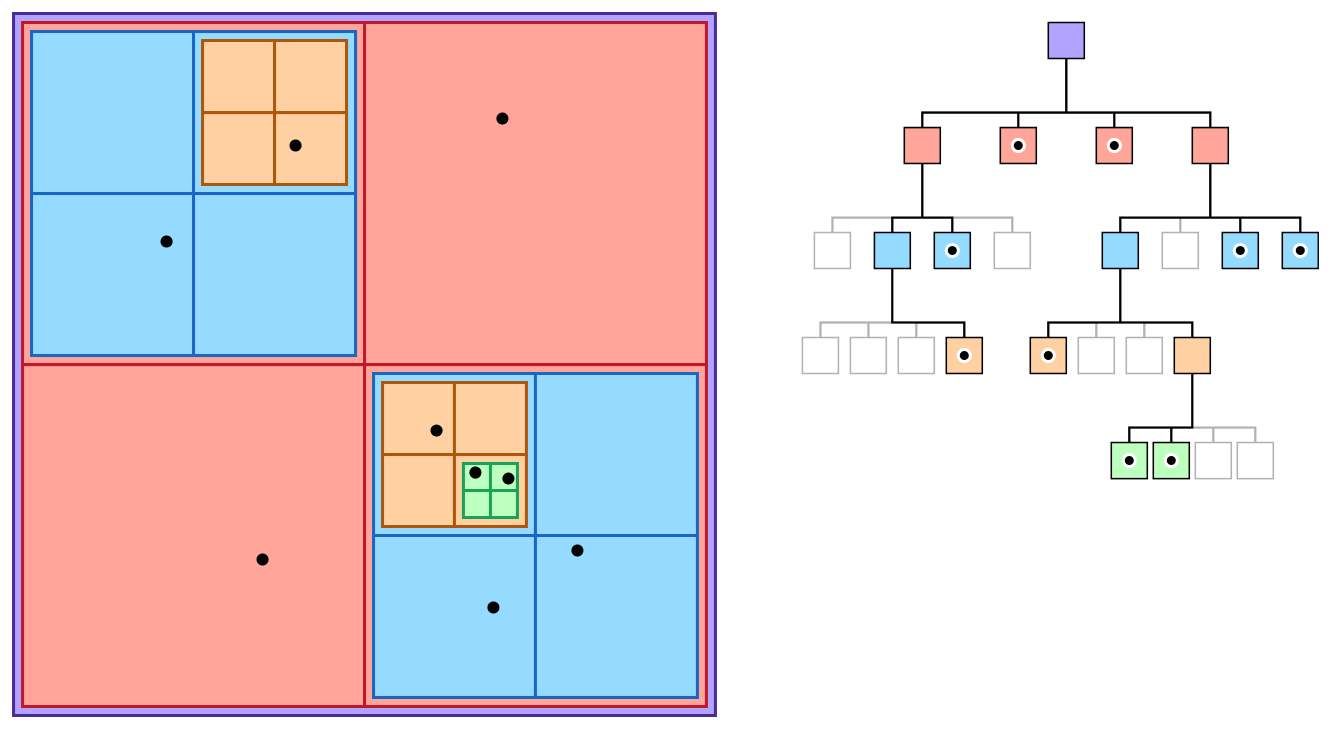
\includegraphics[width=0.7\textwidth]{imgs/quadtree.png}
\caption{A 2D quadtree \textit{(source: Apple)}}
\label{quadtree}
\end{figure}

To define a distance on $Q(X)$, we say that the edge between a node of depth $d$ and a node of depth $d+1$ has weight $2^{\log(\Phi)-d}$. We consider the root to be of depth $0$, thus the edges between the root and its children have weight $2^{\log(\Phi)}$. The distance $t$ between two leaves is then defined as the sum of the weights of each edges present along the unique path between the two leaves. As appendix A.2 of \cite{Flowtree} shows, the tree distance $t$ is related to $l_1$ distance, and thus $l_p$ distance by equivalence of norms in finite dimension spaces.

Interestegly, this step doesn't involve the distributions $\mu$ and $\nu$ for which we intend to compute an estimate of $W_1$. We can build the quadtree on $X$ and repeat the steps 2 and 3 for any number of distributions, which is why this algorithm is used for neireast neighboor search. 

\subsection{Computing the optimal flow} \label{ssec:computing_optimal_flow}
Step 2 of Flowtree is computing the solution of Kantorovitch problem in regards to $Q(X)$, $\mu$ and $\nu$:
$$
f^* = \underset{f \in \mathcal{M}(\mu, \nu)}{\text{argmin}} \sum_{(x, x') \in Q(X)^2} t(x, x') f(x, x')
$$
where $\mathcal{M}(\mu, \nu) = \lbrace f \in \mathcal{M}_+(X, X),~ p_1(f) = \mu,~ p_2(f) = \nu \rbrace$ is the set of distributions over $X^2$ with $\mu$ and $\nu$ as marginals. The elements of this set are called \textbf{flows} and $f^*$ is the \textbf{optimal flow}.\\
Here lies the interest of $Q(X)$, because $f^*$ can be computed exaclty with complexity $\mathcal{O}(s(d+h))$ where $h$ is the height of $Q(X)$ and $s$ is an upper bound for the size of the supports $\mu$ and $\nu$.

To do this, we first turn $Q(X)$ into a tree $D(X, \mu, \nu)$ that we'll call the demand tree, for reasons that will become apparent later. We define $D(X, \mu, \nu)$ by taking $Q(X)$ structure (we leave all nodes intact) and replacing the content of each leaf. Recall each leaf has an index $(i)$ because it corresponds to an element $x_i$ of $X$. Leaf $(i)$ in the quadtree becomes leaf 
$( \lbrace \mu_i \triangleq \mu(x_i) \rbrace , \lbrace \nu_i \triangleq \nu(x_i) \rbrace )$ 
in the demand tree. We call set $\lbrace \mu_i \rbrace$ the $\mu$-demand and same goes for $\nu$. This process is visible in figure \ref{qtree_distrib_ftree}.

\begin{figure}[h]
\centering
\includegraphics[width=0.78\textwidth]{imgs/qtree_distrib_ftree.png}
\caption{How the demand tree is formed}
\label{qtree_distrib_ftree}
\end{figure}

In practice, since the support of $\mu$ and $\nu$ are bounded by $s$, 
many of these leaves become leaf $(\emptyset, \emptyset)$, 
as is the case with leaf $(3)$ in table \ref{table:flow_computation}. 
To compute the optimal flow, we begin with an emtpy flow $f=0$. We then traverse the demand tree in postorder, which means that we only visit a node after passing through all of its children. When visiting node $N$:

\begin{enumerate}[topsep=0pt,itemsep=-1ex,partopsep=1ex,parsep=1ex]

\item If node $N = (N_\mu, N_\nu)$ is equal to $(\emptyset, \cdot)$ or $(\cdot, \emptyset)$, we stop there and kick the (eventual) remaining demand to the parent node.

\item Since the $\mu$-demand $N_\mu$ (resp. the $\nu$-demand $N_\nu$) isn't empty, $\exists i$ (resp. $j$) such that $\mu_i = \min N_\mu$ (resp. $\nu_j = \min N_\nu$). We compute these indices and the quantity $d = \min (\mu_i, \nu_j)$.

\item We then update the demand of node $N$ with $\mu_i := \mu_i - d$ and $\nu_j := \nu_j - d$ 

\item We update the flow with $f(x_i, x_j) := f(x_i, x_j) + d$.

\item Go back to step 1.

\end{enumerate}

\begin{table}[H]
\centering
\begin{tabular}{c|c} 
\Tree[.{$D(X, \mu, \nu)$} [. [.{$\mu_2 = 0.2$ \\ $\nu_2 = 0.2$} ]
                             [.{$\mu_5 = 0.5$ \\ $\nu_5 = 0.3$} ]]
                          [. [.{$\mu_1 = 0.1$ \\ $\nu_1 = 0.5$} ]
                             [.  [
               	                 [.{$\emptyset$} ]
               	                 [.{$\mu_4 = 0.2$} ]]]]]
&
\hspace{20pt} ~
\Tree[.{$D(X, \mu, \nu)$} [. [.{$\emptyset$} ]
                             [.{$\mu_5 = 0.2$} ]]
                          [. [.{$\nu_1 = 0.4$} ]
                             [.  [
               	                 [.{$\emptyset$} ]
               	                 [.{$\mu_4 = 0.2$ } ]]]]]
\\
\begin{tabular}{ |c|ccccc| } \hline
f & 1 & 2 & 3 & 4 & 5 \\ \hline
1 & 0 & 0 & 0 & 0 & 0 \\ 
2 & 0 & 0 & 0 & 0 & 0 \\ 
3 & 0 & 0 & 0 & 0 & 0 \\ 
4 & 0 & 0 & 0 & 0 & 0 \\ 
5 & 0 & 0 & 0 & 0 & 0 \\ \hline \end{tabular} 
&
\begin{tabular}{ |c|ccccc| } \hline
f & 1 & 2 & 3 & 4 & 5 \\ \hline
1 & 0.3 & 0 & 0 & 0 & 0 \\ 
2 & 0 & 0.2 & 0 & 0 & 0 \\ 
3 & 0 & 0 & 0 & 0 & 0 \\ 
4 & 0 & 0 & 0 & 0 & 0 \\ 
5 & 0 & 0 & 0 & 0 & 0.3 \\ \hline \end{tabular} \\
\\ \hline \\
\Tree[.{$D(X, \mu, \nu)$} [. {$\mu_5 = 0.2$} ]
                          [. {$\mu_4 = 0.2$ \\ $\nu_1 = 0.4$} ]]
\hspace{18pt} ~~
&
\Tree[.{$D(X, \mu, \nu)$} [. {$\mu_5 = 0.2$} ]
                          [. {$\nu_1 = 0.2$} ]]
\hspace{15pt} ~
\\
\begin{tabular}{ |c|ccccc| } \hline
f & 1 & 2 & 3 & 4 & 5 \\ \hline
1 & 0.3 & 0 & 0 & 0 & 0 \\ 
2 & 0 & 0.2 & 0 & 0 & 0 \\ 
3 & 0 & 0 & 0 & 0 & 0 \\ 
4 & 0 & 0 & 0 & 0 & 0 \\ 
5 & 0 & 0 & 0 & 0 & 0.3 \\ \hline \end{tabular}
&
\begin{tabular}{ |c|ccccc| } \hline
f & 1 & 2 & 3 & 4 & 5 \\ \hline
1 & 0.3 & 0 & 0 & 0 & 0 \\ 
2 & 0 & 0.2 & 0 & 0 & 0 \\ 
3 & 0 & 0 & 0 & 0 & 0 \\ 
4 & 0.2 & 0 & 0 & 0 & 0 \\ 
5 & 0 & 0 & 0 & 0 & 0.3 \\ \hline \end{tabular} \\
\\ \hline \\
\Tree[.{$D(X, \mu, \nu)$} [. {$\mu_5 = 0.2$ \\ $\nu_1 = 0.2$ } ]] \hspace{25pt} ~~
&
\Tree[.{$D(X, \mu, \nu)$} [. {$\emptyset$} ]] \hspace{18pt} ~~
\\
\begin{tabular}{ |c|ccccc| } \hline
f & 1 & 2 & 3 & 4 & 5 \\ \hline
1 & 0.3 & 0 & 0 & 0 & 0 \\ 
2 & 0 & 0.2 & 0 & 0 & 0 \\ 
3 & 0 & 0 & 0 & 0 & 0 \\ 
4 & 0.2 & 0 & 0 & 0 & 0 \\ 
5 & 0 & 0 & 0 & 0 & 0.3 \\ \hline \end{tabular}
&
\begin{tabular}{ |c|ccccc| } \hline
f & 1 & 2 & 3 & 4 & 5 \\ \hline
1 & 0.3 & 0 & 0 & 0 & 0 \\ 
2 & 0 & 0.2 & 0 & 0 & 0 \\ 
3 & 0 & 0 & 0 & 0 & 0 \\ 
4 & 0.2 & 0 & 0 & 0 & 0 \\ 
5 & 0.2 & 0 & 0 & 0 & 0.3 \\ \hline \end{tabular}
               		
\end{tabular}
\caption{Optimal flow computation for the demand tree described in \ref{qtree_distrib_ftree}}
\label{table:flow_computation}
\end{table}

To understand this algorithm, it helps to think in term of offer and demand. Say $\mu$ is the distribution of producers of a goods (offer) and $\nu$ is the distribution of demanders of goods (demand). If offer and demand exist in the same place, ie on the same node, then we can do the exchange in that place (step 4) and we keep track of the exchange made (step 5). This exchange has to be small enough for both the producer and the demander, thus we look for the minimal exchange (step 3). Otherwise (stop case of step 1), we have to move the goods, which corresponds to kicking the demand (both in term of producers and demanders) to the parent node.\\
In this example, the $\mu$-demand is called the offer and the $\nu$-demand the demand, but in the general case, both are called demands. One can think of the $\mu$-demand (the offer) as a demand for buyers, and the $\nu$-demand (the demand) as a demand for sellers. \\
To illustrate this algorithm, we can refer to table \ref{table:flow_computation}.

Although we written the $\mu$-demand as a set $\lbrace \mu_i, \dots \rbrace$ to save time, we do need to keep track of both $i$ and the associated quantity $\mu_i$. More on that in part \ref{ssec:DataSctructures}. 

\subsection{Compute $W_1$ estimate}
We now compute the $W_1$ estimate using the optimal flow $f^*$ computed on $D(X, \mu, \nu)$. The logic here is that since $f^*$ is the optimal argument to the Kantorovitch problem defined by the tree distance, itself an approximation of the $l_p$ distance, then using $f^*$ as an argument for the Kantorovitch problem defined by the $l_p$ distance will yield a near-optimal value.\\

This final step is quite simple: we just have to sum over the couples for which $f^*$ is non-zero the optimal flow value times the distance of the two points to get the estimate $\widetilde{W}_1$ of $W_1$:

$$
\widetilde{W}_1(\mu, \nu) = \sum_{(x, x') \in S^*} f^*(x, x') \Vert x - x' \Vert_p
$$ 

with $S^*$ the support of $f^*$.

\section{Technical details}

\subsection{Fusing step 2 and 3} \label{ssec:fuse23}
Since the only use of $f^*$ is to be used for the computation of $\widetilde{W}_1(\mu, \nu)$, one can fuse the step 2 and 3 of the algorithm by not computing $f^*$ but incrementaly increasing $\widetilde{W}_1(\mu, \nu)$ during step 2. We remove step 3 and replace at sub-step of step 2:

4. We update the flow with $f(x_i, x_j) := f(x_i, x_j) + d$.
\\
with:

4. We update the estimate with $\widetilde{W}_1(\mu, \nu) := \widetilde{W}_1(\mu, \nu) + d \Vert x_i - x_j \Vert_p $.
\\
We can go further add memoïze the distances $\Vert x_i - x_j \Vert_p$ as we compute them and decrease the computationnal cost (by increasing the memory cost).

\subsection{Data structures}\label{ssec:DataSctructures}
As we mentionned ealrier, given a node $N$ with $\mu$-demand and $\nu$-demand, we need to keep track of $i$ and $\mu_i$ (same goes for $\nu$). Thus, we uset an array with 3 columns: index $i$, $\mu_i$ and $\nu_i$. Each node as an array and the algorithm finishes when the root has been visited and its array is empty. If it isn't, then there was an error during the computation of $f^*$. For instance, this happens if the distribution's masses were not normalized to $1$ or if there is no tolerance for floating-point error. To avoid this, we consider values to be equal to zero when they fall behind $10^{-12}$. Original implemenation \cite{FlowtreeGit} has $10^{-8}$ but we haven't had any problem with our value.\\ 
For distributions, we used a dictionnary-like data structure that returns $0$ when we try to access a value that isn't in the dictionnary. This is optimal because distributions are only used to access values and check if a value is in the support, both of which are $\mathcal{O}(1)$ operation with dictionnaries.\\
Since we fused step 2 and 3 in subsection \ref{ssec:fuse23}, we need not worry about the data structure of $f^*$, but if for some reason we still wanted to keep the optimal flow (e.g. to try different norms other than the norm 2 in $\widetilde{W}_1$) a dictionnary with default value $0$ is best, as all operations done on it are in $\mathcal{O}(1)$ complexity.

\subsection{Hypercube splitting}
In \ref{ssec:building_the_quandtree}, we defined the split operator on a hypercudbe $H(x, l)$. One can wonder how this is done in practice, as we did when we implemented the Flowtree algorithm. Since we discard the sub-hypercube $H(x_{b_1 \dots b_d}, l/2)$ that intersect no point in $X$, we take advantage of this. We reverse the process: before creating a sub-hypercube, we look if it will contain a point of $X$, and only create it if its the case.\\
Given an hypercube $H(x, l)$ that contains a subset $Y$ of $X$, we compute $m = (x_1+l/2, \dots, x_d+l/2)$ the "middle" of the hypercube. Then, for each $y$ of $Y$, we compute $b = (b_1, \dots, b_d)$ the boolean vector defined by $b_i = 1$ if and only if $y_i \leq m_i = x_i + l/2$. This can be done quickly by rearranging $Y$ into a matrix of dimension $\vert Y \vert \times d$ an do a vectorized comparaison with $m$. 
This results in a boolean matrix $B$ of size $\vert Y \vert \times d$. Each line of $B$ corresponds to a point $y$ and describes the sub-hypercube in which $y$ will be: $y \in H(m + \frac{l}{2}b, l)$.
We have an association from point to sub-hypercube $f: y \rightarrow b$ and need to group points by sub-hypercube. We just reverse $f$ with a dictionnary ($b$ can be stored as bytes to ensure hashability) where keys are $b$ and values $f^{-1}(b)$. This can be done by iterating through the $B$ and costs $(\mathcal{O}\vert Y \vert d)$. Then for each key $b$, if $f^{-1}(b)$ isn't a singleton create an hypercube, otherwise create a leaf.\\

\section{Theoretical garantees}

\subsection{Complexity of Quadtree building}\label{ssec:ComplexityQuadtreeBuilding}
So as to go with the flow of the paper, we will split the complexiy analysis in two part. As the Flowtree algorithm is meant for nearest neighboor search, the Quadtree $Q(X)$ needs only to be built once, and the computation of $\widetilde{W}_1$ is meant to be repeated for many distributions. Here, we will only cover the cost of buildin $Q(X)$.\\
The paper advertises the cost of building $Q(X)$ as $\widetilde{\mathcal{O}}(\vert X \vert d \log(d\Phi))$. 
However, it makes two hypothesis on the data $X$: non-negative coordinates and $\min_{(x, x') \in X^2} \Vert x - x' \Vert = 1$. 
The former is easy to guarantee by offsetting $X$ by its minimal coordinate, which can be done in time $\mathcal{O}(\vert X \vert d)$.
The latter is however harder to achieve. It's unclear which norm is used, but regardless of whether it is $\Vert \Vert_1$ or any $\Vert \Vert_p$, computing the maximal distance plus scaling costs $\mathcal{O}(\vert X \vert^2 d)$. Furthermore, this factor can be quite large. Suppose the minimal distance is proportionnal to $2^{-\vert X \vert}$, as is the case in \ref{worst_case_qb}, then $\Phi$ implicitely carries the inverse of this factor, since it's the maximal coordinnate \textbf{after} scaling $X$, so $\log(d\Phi) = \mathcal{O}(\vert X \vert \log(d))$. This is in my opinion one of the weak point of the paper: the fact that the minimal distance is reduced to $1$ is actually a big assumption and has an impact on any complexity analysis where $\Phi$ appears.\\
Plus, in parctice, it seems\footnote{source: discussing this with Gabriel Peyré} is skipped, as it's quite heavy. This doesn't mean that the problem due to $\Phi$ disappears, because then the complexity of $Q(X)$'s construction can't be bounded in the same way the paper does.

\begin{figure}[h]
\centering
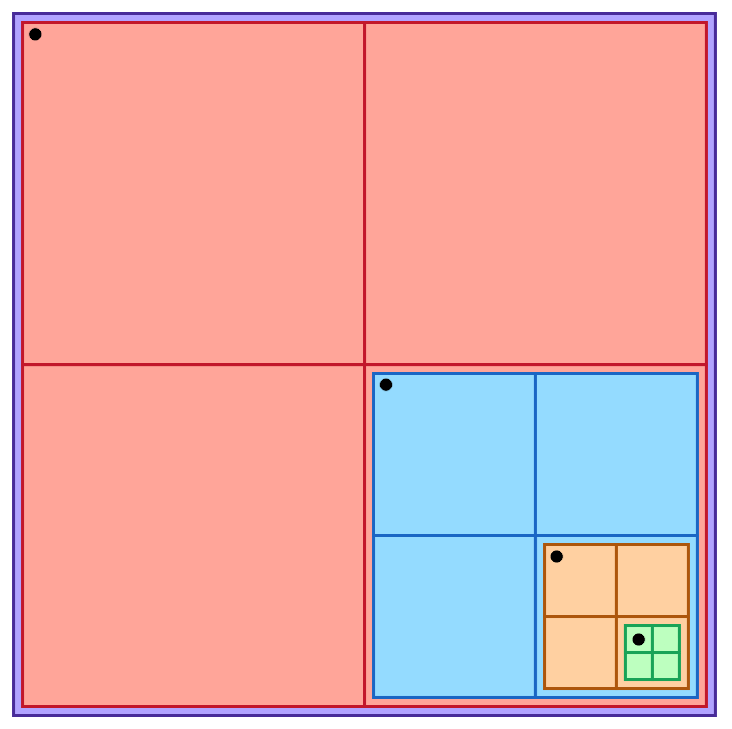
\includegraphics[width=0.35\textwidth]{imgs/worst_case_qb.png}
\caption{An set $X$ where the minimal distance is inversly exponnetial to $\vert X \vert$}
\label{worst_case_qb}
\end{figure}

To simplify further complexities, we will still assume this minimal distance normalization has been done, but we will do well to keep in mind this could add complexity whenever $\Phi$ appears. With that hypothesis, since the minimal size of the Quadtree cell is bounded, $Q(X)$ height $h$ is bounded too and $h = \mathcal{O}(log(\Phi d))$.

\subsection{Complexity of $\widetilde{W}_1$ estimation}
In this subsection, we suppose we've built the $Q(X)$. The next step is to compute $D(X, \mu, \nu)$ which requires copying $Q(X)$ and introducing demand for each node.\\
Notice that demand tree nodes are only used if at least one of their child is a leaf $(i)$ such that $i \in \supp(\mu) \cap \supp(\nu)$. By traversing $Q(X)$ in preorder, we can apply this and only copy the nodes that verify this, we just have to backpropagate a boolean by node that's only true if the node or one of its chlidren is a leaf in the support. Since the supports of $\mu$ and $\nu$ are supposed to be bounded by $s$, there are at most $2s$ leafs that verify this, and $2sh$ nodes that verify this. The demand introduced at this step is either a $3 \times 1$ or $3 \times 0$ array with constant build-time.\\
We deduce the complexity of building $D(X, \mu, \nu)$ is $\mathcal{O}(sh)$. We now need to compute the optimal flow from it. Each echange (step 3 of the algorithm in \ref{ssec:computing_optimal_flow}) cancels either $\mu_i$ or $\nu_j$, so this happens at most $2s$ times. When such an exhange happens, we also need to compute $\Vert x_i - x_j \Vert_p$, so the total complexity of all exhanges is $\mathcal{O}(sd)$. To carry out all exhanges, we need to traverse the whole tree, so we add a complexity of $\mathcal{O}(sh)$ to get a complexity of $\mathcal{O}(s(d+h))$. Using the order of magnitude of $h$ computed at the end of \ref{ssec:ComplexityQuadtreeBuilding}, we end up with a complexity of $\mathcal{O} \left(s \left(d+\log(d\Phi)\right) \right)$

\subsection{Accuracy of $\widetilde{W}_1$ estimation}
We now tackle the problem of estimating $\widetilde{W}_1$ accuracy when compared to $W_1$. Using the same notations as before, right of the bat we can notice that

$$
W_1(\mu, \nu) 
= \min_{\tau} \sum_{\left( x, x' \right) \in X^2 } \tau(x, x') \Vert x - x' \Vert_p
~\leq~ \sum_{\left( x, x' \right) \in X^2 } f^*(x, x') \Vert x - x' \Vert_p
= \widetilde{W}_1(\mu, \nu)
$$

so the Flowtree estimate will always sit above the actual $W_1$ value. For this reason, in part \ref{sec:Numerics}, we will always look at the ratio $\widetilde{W}_1 / W_1$ to review the performance of Flowtree.\\

One of the paper's flaw, in my opinion, is that it only gives accuracy guarantee for $\widetilde{W}_1$ in the context of nearest-neighbor search. Although, when proving this guarantees, the paper gives a guarantee on the quality of $\widetilde{W}_1$ in regards to $W_1$.\\
In proof of \cite{Flowtree} theorem 3.4, it is shown that for the optimal flow $\tau^*$ according to $W_1$ we have:

$$
\widetilde{W}_1(\mu, \nu) 
= \sum_{\left( x, x' \right) \in X^2 } f^*(x, x') \Vert x - x' \Vert_1 
~\leq~ \mathcal{O}(\log(s)) \sum_{\left( x, x' \right) \in X^2 } f^*(x, x') t(x, x')
$$

From this, we can re-introduce $\tau^*$ because the optimal flow $f^*$ is optimal for the tree metric $t$:

$$
\mathcal{O}(\log(s)) \sum_{\left( x, x' \right) \in X^2 } f^*(x, x') t(x, x')
~\leq~ 
\mathcal{O}(\log(s)) \sum_{\left( x, x' \right) \in X^2 } \tau^*(x, x') t(x, x')
$$

We now use:

$$
\sum_{\left( x, x' \right) \in X^2 } \tau^*(x, x') t(x, x') 
~\leq~ 
\mathcal{O}(\log(d\Phi)) \sum_{\left( x, x' \right) \in X^2 } \tau^*(x, x') \Vert x - x' \Vert_1 = \mathcal{O}(\log(d\Phi)) W_1(\mu, \nu)
$$

Combining all this, we get:

$$
W_1(\mu, \nu) 
~\leq~ 
\widetilde{W}_1(\mu, \nu)
~\leq~ 
\mathcal{O}(\log(s) \log(d\Phi)) \cdot W_1(\mu, \nu)
$$

This back and forth between $f^*$, $\tau^*$, $t$ and $\Vert \Vert_1$ is the proof's keystone. One can notice that here, we used the $l_1$ norm instead of general $l_p$ norm, but since we are working inside a finite dimensions, these norms are equivalent and this adds a constant factor squarred in the $\mathcal{O}$. \\

The paper even shows that for uniform distributions, we can lower the inside of $\mathcal{O}$ to $\log \left( s \right)^2$, which doesn't make $\Phi$ appear. However, we have tried to determine if that bound is reliant on the assumption that the minimal distance has been reduced to 1, but this is unclear. In any case, at the cost of this (expensive) pre-processing, which can be agreable to in the case of nearest-neighbor search, the bound holds and is quite enticing.

\newpage
\section{Numerics}\label{sec:Numerics}

In this section, we'll benchmark to quality of the Flowtree approximation by looking at the ratio $\widetilde{W}_1 / W_1$ where $W_1$ is computed with the \textsf{POT} \cite{POT} package, which uses the algorithm proposed in \cite{POTalgo}.

\subsection{Spherical model}

\subsubsection{Description of the model}

The first model we're going to test the Flowtree algorithm on is similar to the one used in the paper. We choose a dimension $d$ and a number of points $N$ and draw each element of $X$ by following this process:

\begin{enumerate}
\item Draw a vector $\tilde{x}$ where each component is in $\mathcal{U}(-1, 1)$
\item Add noise by drawing $\sigma$ in $\mathcal{N}(1,~ 0.04)$
\item Keep the noisely-normalized vector $x = \sigma \tilde{x} \Vert \tilde{x} \Vert^{-1}_2$
\end{enumerate}

We then draw uniformely two distribution $\mu$ and $\nu$ on $X$ with support size $s$ and uniform weights. This is visible in figure \ref{spherical_repr}. One could ask themselves if collisions (i.e., repeated values in the dataset) are likely to happen: not at all, since numbers generated are 64-bit floats: the chances of collisions are $2^{-64*d}$.

\begin{figure}[h]
\centering
\includegraphics[width=0.5\textwidth]{imgs/spherical_repr.png}
\caption{Two distributions drawn with the spherical model}
\label{spherical_repr}
\end{figure}

The noise was initially added to make for a prettier figure, since it allowed for the sampled points not te be all superposed. For this reason, we kept it, since it helps the distribution to be less concentrated on the unit sphere. In the end, the model has 3 parameters: $(d, N, s)$.

\subsubsection{Dependance on the $l_p$ norm chosen}
The paper is quite vague about which norm is chosen in $\R^d$ to compute the Wasserstein distance. In their implementation \cite{FlowtreeGit}, the authors only compute the Flowtree estimate using the $l_2$ norm. However, there is no apparent reason for this, so we've took a look at the impact of the $l_p$ norm on the $\widetilde{W}_1 / W_1$ ratio. This can be seen in figure \ref{spherical_boxplots} where $(d, N, s) = (2, 40000, 400)$.

\begin{figure}[h]
\centering
\includegraphics[width=1\textwidth]{imgs/spherical_boxplots_ratio_p.png}
\caption{Impact of $p$ (in $l_p$) on the $\widetilde{W}_1 / W_1$ ratio}
\label{spherical_boxplots}
\end{figure}

Interestingly enough, it seems the estimation gets better as $p$ goes up, but this trends plateaus for $p \geq 2$. However, there is a noticeable difference between $p=1$ and $p=2$, and the estimation gets much worse when $p=0.5$. This might be because the distance defined by the $l_p$ norm gets closer to the tree distance when $p$ increases.\\
Since $p=2$ corresponds to the euclidian norm and the estimate is almost as good as it gets and close the $p=1$ estimate, we'll use $l_2$ as the norm in the rest of the numerics unless specified.

\subsubsection{Dependance of the estimate on the dimension}
Now we've decided on which $l_p$ norm to use ($l_2$), we take a look at the impact of $(d, N, s)$ on the estimate's quality. We're going to fix $(N, s)$ and monitor the $\widetilde{W}_1 / W_1$ ratio as $d$ changes.\\
For the choice of $(N,s)$, we take two couples from the paper: $(100, 10)$ and $(1000, 100)$, add a couple in the middle $(500, 10)$ and two larger models $(5000, 100)$ and $(10000, 400)$.\\
For the range of $d$, we sample low dimension more than high dimension and set $d \in \lbrace 2, 3, 5, 10, 20, \dots, 100 \rbrace$.\\

\begin{figure}[h]
\centering
\includegraphics[width=0.8\textwidth]{imgs/spherical_ratio_by_d_v2.png}
\caption{Impact of dimension on the $\widetilde{W}_1 / W_1$ ratio, spherical model}
\label{spherical_ratio_by_d_v2}
\end{figure}

Interestingly, the quality of the estimate does not depend on $N$ but only on $s$. This is essentialy what theorem 3.6 in \cite{Flowtree} ensures. We will see that this still holds for other models, as fig. \ref{gaussian_quality_by_dim} shows. Interestingly, initially the estimate gets worse as dimension grows, until $d=7-10$ and then gets progressively better. It is best for very large dimensions. 

\newpage
\subsection{Gaussian model}

\subsubsection{Description of the model}
Now, we try a model where distributions are not uniform. We again choose a triplet $(d, N, s)$ for the dimension, number of points and support size, again draw $X$ and $\mu$ in the following way:

\begin{enumerate}
\item Draw a vector $\tilde{x} \in \R^d$ where each component is in $\mathcal{N}(0, 1)$
\item Add vector $x = A\tilde{x}$ to $X$: $x$ follows $\mathcal{N}(0, AA^T)$
\item Add $x$ to $\supp(\mu)$ with $\mu(x) = \Vert \tilde{x} \Vert_2$
\item Repeat step 1-3 until $\vert X \vert = N$ and randomly (uniformly)  truncate $\supp(\mu)$ so $\vert \supp(\mu) \vert = s$
\end{enumerate}

This leads to the kind of distributions shown in figure \ref{gaussian_repr} where points near the center of the gaussian are heavier than other.

\begin{figure}[h]
\centering
\includegraphics[width=1\textwidth]{imgs/gaussian_repr.png}
\caption{Gaussian distributions with $(d, N, s) = (2, 10000, 800)$. Colors are normalized: red (resp. blue) is the distribution's maximum (resp. minimum) and grey points are outside of the support.}
\label{gaussian_repr}
\end{figure}

Since we want to go from one distribution $\mu$ to another $\nu$, we need two distributions one the same support. We chose the draw each with $(d, N/2, s)$ and fuse the sets of points on which they were drawn. This means that each distribution has 'less' than $N$ points on which it can be non-zero, but rather $N/2$. 
This leads to the model seen in figure \ref{gaussian_repr_2}

\begin{figure}[h]
\centering
\includegraphics[width=1\textwidth]{imgs/gaussian_repr_2.png}
\caption{Two gaussian distributions as in fig. \ref{gaussian_repr} with $(d, N, s) = (2, 10000, 800)$. Colors are normalized and grey points are outside of the support.}
\label{gaussian_repr_2}
\end{figure}

\subsubsection{Dependance on dimension}
As for the spherical mode, we fix $(N, s)$ and vary $d$ to see its impact on the ratio. We chose $(N,s)$ so that the independance on $N$ and dependance on $s$ appeared.

\begin{figure}[h]
\centering
\includegraphics[width=0.8\textwidth]{imgs/gaussian_quality_by_dim.png}
\caption{Impact of dimension on the $\widetilde{W}_1 / W_1$ ratio, gaussian model}
\label{gaussian_quality_by_dim}
\end{figure}

Once again, we see that $s$ impacts $\widetilde{W}_1 / W_1$ but $N$ does not. We also see that the curve has the same aspect as the one in figure \ref{spherical_ratio_by_d_v2}. This could suggest that we could enhance the estimate's quality by trying to predict the ratio depending on $(d, s)$. 

\subsubsection{Empirical time cost analysis}
Now we've compared the accuracy of Flowtree, it would be interesting to compute its speed. To do that, we are going to go with a very basic comparaison scheme, just look at the mean time taken to compute $\widetilde{W}_1 $ and $W_1$ depending on the dimensions for $(N, s) \in \lbrace (100, 10), (1000, 100), (10000, 400) \rbrace$. The result can be seen on the left graph of figure REF.

\begin{figure}[h]
\centering
\includegraphics[width=1\textwidth]{imgs/gaussian_time_by_dim.png}
\caption{Time cost analysis of Flowtree (ours) and POT}
\label{gaussian_time_by_dim}
\end{figure}

Let's adress the elephant in the room: the fact that our implementation of Flowtree is much (10x times) than POT is disappointing. But, since POT is a library maintained by at least 50 top-notch academicals and has been around for 7 years, this is not surprising. I surmise the culprits for the efficiency of POT are parallelisation (processes and CPU cores) and lazy evaluation of the distance matrix. Especially because the computation of the right graph took an enormous amount of time, and involved the search of the minimum coefficient of the distance matrix, thus forcing evaluation of all its coefficients. Because of time constraint, I didn't have time to code Flowtree in a more efficient way, which would have involved C++. We can keep in mind that once again, regardless of the algoirthm we choose, the main speed bottleneck is carefull implementation and hardware.\\
For theoritical costs of the methods involved, we better refer ourselves to subsection \ref{ssec:PreviousWorks}.\\

Nevertheless, this figure has some merit. As we can see, lower dimension are the ones where the time cost of Flowtree is the highest, which could seem illogical. But actually, this makes sense, since the complexity of building $Q(X)$ goes up as points of $X$ get closer, because it takes more hypercubes splitting. This is what we've talked about in \ref{ssec:ComplexityQuadtreeBuilding}: the complexity of Flowtree depends on the minimal distance of the points in $X$, which is baked in $\Phi$ when you assume the minimal distance to be $1$. 


\section{Conclusion}

\subsection{On Flowtree}
In the end, Flowtree seems a reliable algorithm to predict $W_1$ on several distrbutions support on a single set.\\
The bulk of the algorithm's cost is paid only once per set, and the subsequent computations of $W_1$'s estimate for pairs of distributions are much less expensive.  This is one of the main edge of Flowtree, and the reason it was made for nearest neighbor search. The other main guarantee on Flowtree is that its performance does not degrade as the set of points $X$ grows. We witnessed this firsthand in our experiments, as the numerics show.\\

However, the algorithm can struggle when the set of points on which the Quadtree is built contains lots of close points, and this is overlooked by the paper as it assumes the minimal distance to be 1: this is what we saw in the low-dimension gaussian models. This can lead to hidden complexity in practice, and the addition of the smallest distance in the complexity analysis would make them more realistic. But it's not a mistake in the strict sense of the word, as everything in the paper stands if a preprocessing cost of $\mathcal{O}(\vert X \vert^2 d)$ is done.\\
Apart from this, the paper is quite well written and thorough, but it would have been nice to mention some bounds on the quality of $W_1$ estimate instead of limiting itself to the notion of $c$-nearest neighbor estimate.\\

One think to keep in mind is that this algorithm is not meant to be used to compute $W_1$. It should be used to compute an estimate in situations where algorithms more precise take too long. This is why the paper uses Flowtree in nearest-neighbor pipelines. But, for the sake of benchmarking, the quality of $W_1$'s estimation is the angle under which we studied Flowtree in this report, which turned out to be worthwhile.

\subsection{Possible improvements}

\subsubsection{Estimating $\widetilde{W}_1 / W_1$ depending on $(s, d)$}
As we've seen with the Spherical model and Gaussian model in figures \ref{spherical_ratio_by_d_v2} and \ref{gaussian_quality_by_dim}, it seems that for a fixed model, the ratio of $\widetilde{W}_1 / W_1$ can be estimated using only $s$ and $d$. Thus we could possibly decrease the gap between the estimate and the actual $W_1$ distance with little to no cost, if however we can reliably predict the ratio. This could lead to an improvement of the algorithm, and is perfectly applicable in the context of the nearest-neighbor search problem. 

\subsubsection{Maximal density of Quadtree leaf}
Another possibly fruitfull avenue would be to define a threshold for the minimal size of Quadtree leaves. If the dataset is really dense in a leaf, rather than dividing said leaf until we had tiny leaves with one point each, we could assign several point to an already small leaf and save the computations. That could prove advantageous in terms of complexity of computing both the Quadtree and the optimal flow, as these steps's complexity depends on the Quadtree's height and thus the minimal distance between points. This wouldn't change the algorithm in any major way, so it would be easy to implement and test. It would especially be worthwhile for dataset where density of points vary a lot and rise high.

\section{Connetions with the course}
The main notion that links this paper to the Optimal Transport course is evidently the Wassertein distance. We have seen that this function is indeed a distance for $p \geq 1$, and from the course notes, it seems the results holds for $p=1$. Although during class we could not delve deep into the property of $W_p$, we did see a theorem stating that $W_1$ can be seen as a norm on distribution differences and computed with a supremum over Lipschitz function of Lipschitz constant 1. Although I'm not sure how this could be used to computed $W_1$ effectively, it sures would be fun to try.\\

% Kantorovitch problem
In the course, we introduced $W_1$ after talking about Sinkhorn's algorithm, which is used to solve Schrodinger's problem. As it is a relaxation of Kantorovitch, it can be applied to $W_1$ in our context. Hence, we can see that any Kantorovitch solution or Schrodinger solution can be applied to the computation of $W_1$, as stated in \ref{ssec:PreviousWorks}. Thus, algorithms we saw in class are relevant to this problem.\\
% Linear program and simplexes
First, since Kantorovitch is a linear program, simplex method would work in our case, our even better network simplexes. Second, interior points methods like Nesterov and Nemirowski, which we talked about in class and did a numerical tour on, would also be pertinent.\\

% Sinkhorn
Finaly, as we mentionned before, Sinkhorn algorithm, that we studied in class, is also apropos to the computation of $W_1$, even moreso than the algorithms talked about before. However, we've seen its complexity, which makes Sinkhorn quite expensive to use in the context of nearest neighbor search. 




\end{document}
